\documentclass[laboratorio]{guia}

\def \practnum {9}
\def \practica {Difracci\'on de la luz}

\def \materia {Laboratorio de F\'\i sica II para Qu\'\i micos}
\def \periodo {2do. Cuatrimestre de 2015}
\def \catedra {Pablo Cobelli}
\def \website {http://materias.df.uba.ar/f2qa2015c2}

\usepackage{graphics}
\usepackage{amsmath}
\usepackage{amsfonts}
\usepackage{graphicx}
\usepackage{float}
\usepackage{wrapfig}
\usepackage{subfigure}
\usepackage{bm}
\usepackage{grffile}
\usepackage{color}
\usepackage{framed}
\usepackage[utf8]{inputenc}
\usepackage[T1]{fontenc}
\usepackage{lmodern}
\usepackage{circuitikz}
\usepackage[spanish]{babel}
\usepackage{babelbib}
\selectbiblanguage{spanish}



%----------------------------------------------------------
% Agrega al path de figuras el subdirectorio con el mismo
%     nombre que el archivo principal del proyecto
\graphicspath{{./\jobname/}}

%----------------------------------------------------------
% Definicion del entorno 'sabermas'
\makeatletter
\definecolor{shadecolor}{rgb}{0.89,0.91,0.94}
\newenvironment{sabermas}[1]{%
\vfill
\begin{shaded}
  \begin{center}
  {\textsection{Para saber m\'as}}
  \end{center}
  #1
\sf } 
{%
\end{shaded}%
}
\makeatother

%----------------------------------------------------------
% Definicion del entorno 'problema'
\newcounter{ContadorProblema}
\setcounter{ContadorProblema}{0}
\newcounter{TieneFiguraAsociada}
\setcounter{TieneFiguraAsociada}{0}
\newcounter{UbicacionFigura}
\setcounter{UbicacionFigura}{0}

\newenvironment{problema}[2][]
{%
    \ifx\relax#1\relax%
        \setcounter{TieneFiguraAsociada}{0}
        \else
        \setcounter{TieneFiguraAsociada}{1}
    \fi
    \def \archivofigura {#1}
    % 
    \refstepcounter{ContadorProblema}
    \noindent%
    \ifnum\value{TieneFiguraAsociada} < 1%
        {\sffamily \bfseries Problema \arabic{ContadorProblema}.}
        %{\sc {#1}}%
        \par\nobreak\par\nobreak%
        \medskip 
    \else
        % Va con figura; resta determinar de que lado.
        \ifnum\value{UbicacionFigura} < 1
            % Poner la figura del lado derecho
            \begin{minipage}{12.25cm}
            {\sffamily \bfseries Problema \arabic{ContadorProblema}.}
            %{\sc {#1}}%
            \par\nobreak\par\nobreak%
            \medskip 
        \else
            % Poner la figura del lado izquierdo
            \begin{minipage}{4.5cm}
                \centering
                \includegraphics[width=4.5cm]{\archivofigura}
                {\footnotesize {\sffamily Esquema asociado al 
                problema \arabic{ContadorProblema}}.}
            \end{minipage}\hfill%
            \begin{minipage}{12.25cm}
                {\sffamily \bfseries Problema \arabic{ContadorProblema}.}
                %{\sc {#1}}%
                \par\nobreak\par\nobreak%
                \medskip 
        \fi
    \fi
}
{%
    \ifnum\value{TieneFiguraAsociada} < 1%
        % \par \bigskip \vskip 0.3cm
    \else
        % Va con figura; resta determinar de que lado.
        \ifnum\value{UbicacionFigura} < 1
            % Poner la figura del lado derecho
            \end{minipage}\hfill%
            \begin{minipage}{4.5cm}
                \centering
                \includegraphics[width=4.5cm]{\archivofigura}
                {\footnotesize {\sffamily Esquema asociado al 
                problema \arabic{ContadorProblema}}.}
            \end{minipage}
        \else
            % Poner la figura del lado izquierdo
            \end{minipage}%
        \fi
    \fi
    \setcounter{TieneFiguraAsociada}{0}
    \par \bigskip \vskip 0.3cm
    % Permutamos el valor de la ubicacion
    \ifnum\value{UbicacionFigura} < 1
        \setcounter{UbicacionFigura}{1}
    \else
        \setcounter{UbicacionFigura}{0}
    \fi
}

%----------------------------------------------------------
% Definicion/Redefinicion de estilos
\renewcommand{\vec}[1]{\ensuremath{\mathbf{#1}}}


\hyphenation{ coe-fi-cien-tes coe-fi-cien-te au-to-va-lor
              au-to-va-lo-res co-rres-pon-der pro-ble-ma 
              cual-quie-ra po-la-ri-za-cio-nes }

\graphicspath{{./difraccion/}}

\begin{document}
\objetivo{
  Medir la figura de difracción de Fraunhoffer producida por una rendija y por un obstáculo de geometría rectangular, empleando un fotodiodo.
  \tematicas{Difracción de Fraunhoffer, figura de difracción, rendija, medición con fotodiodo.}
  }
\maketitle


\section{Desarrollo de la experiencia}

\subsection{Rendijas y obstáculos; posición de los mínimos}

Iluminando una rendija de ancho variable con un láser de He-Ne, según se muestra en la figura \ref{fig:1} es posible observar, sobre una pantalla lejana, una figura de difracción.

\begin{figure}[ht]
  \centering
  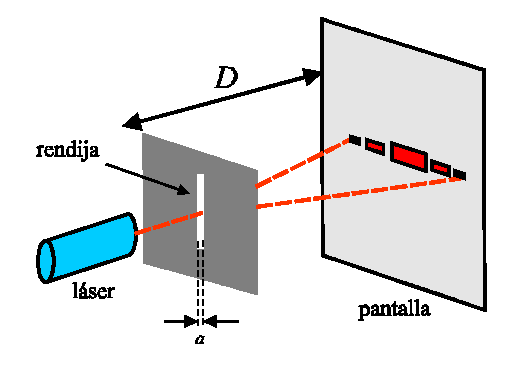
\includegraphics[width=8.5cm]{LG10--000.png}
  \caption{Esquema experimental del dispositivo propuesto para el estudio de la difracción de Fraunhoffer.}
  \label{fig:1}
\end{figure}

Ubique el láser en la mesa óptica asegurándose de que el mismo quede bajo el nivel de las barreras de protección visual.
Remueva sólo una de las mismas y utilice como pantalla la pared.
\textbf{Al trabajar de esta forma, ponga especial atención en no exponer los ojos al haz.} 

Una vez montado el sistema propuesto, observe cómo se distribuye la intensidad de la luz sobre la pantalla.
Investigue la relación entre la distancia entre mínimos (y máximos) de intensidad y el
ancho \(a\) de la rendija. 

A continuación:
\begin{itemize}
  \item Mida la posición de los mínimos \(y_n^\text{mín}\), donde \(n\) denota el orden del mínimo observado, en función de \(n\).
  \item Represente sus resultados en un gráfico.
  \item Sabiendo que
        \begin{equation}
         y_n^\text{mín} = n \frac{D \lambda}{a}, \quad n = \pm 1, \pm 2,
         \ldots,
        \end{equation}
  siendo \(D\) la distancia entre los planos de la rendija y la pantalla, y \(\lambda\) la longitud de onda de la luz empleada, determine el ancho \(a\) de la rendija.
  \item Reemplace ahora la rendija por un alambre (obstáculo) de ancho conocido y estudie en igual manera su figura de difracción.
\end{itemize}

El sistema rendija-obstáculo (cuando presentan ambos un mismo tamaño) se dicen \emph{complementarios}.
Una característica notable de estos sistemas es que forman las mismas figuras de difracción.
Este resultado se conoce como \emph{principio de Babinet}.


\subsection{Distribución de intensidad de las figuras de difracción}

El objetivo de esta parte de la práctica consiste en medir la distribución de intensidad lumínica sobre la pantalla en la que se observan las figuras de difracción.
Para ello, se propone montar sobre una mesa óptica el mismo sistema rendija-láser empleado anteriormente.
Ahora, sin embargo, ubicaremos un fotosensor (fotodiodo) donde antes estaba ubicada la pantalla. 
Resulta conveniente montar el fotodiodo sobre un posicionador traslacional, a fin de poder desplazarlo lateralmente en forma controlada.

El protocolo experimental consiste entonces en desplazar el fotosensor a lo largo de la figura de difracción y registrar, para cada posición, la intensidad local de la luz que a él llega.
El registro de los datos puede realizarse mediante el sistema de adquisición digital SensorDAQ, al cual se encuentra conectado el sensor.
El posicionador dispone de un tornillo micrométrico que permite medir la posición del sensor sobre la figura de difracción. 

En estas condiciones:
\begin{itemize}
  \item Represente los resultados medidos en un gráfico \(I(y)\), es decir, de intensidad observada en función de la posición \(y\) del fotosensor.
  Observe que la teoría predice un comportamiento dado por
  \begin{equation}
    I(y) = I_0 \left(\frac{\sin z(y)}{z(y)} \right)^2,
  \end{equation}
  siendo 
  \begin{equation*}
    z = \frac{\pi a}{\lambda} \sin \alpha(y).
  \end{equation*}
  El ángulo \(\alpha\), que es función de \(y\), mide la apertura angular de la figura de difracción respecto del máximo central, y verifica
  \begin{equation}
    \tan \alpha(y) = \frac{y}{D}.
  \end{equation}
  En este caso, recuerde que si empleó el fotómetro para medir la intensidad, el parámetro \(D\) es la distancia desde el plano de la rendija hasta el elemento sensible del instrumento.
\end{itemize}


\subsubsection*{Observación:}

El fotosensor satura a \SI{3}{\volt}, lo que significa que cuando se lo ilumine con una intensidad superior a la máxima, la lectura que dará el instrumento será siempre de 3 V.
Dadas las características del experimento, y siendo que deseamos observar los máximos de intensidad, es posible que el máximo de orden cero resulte saturado. 



\nocite{Alonso1998,Jenkins2001,Hecht1986}
\bibliographystyle{unsrt} 
\bibliography{Bibliografia}

\end{document}
